\newpage
\section{Auswertung}
\label{sec:Auswertung}
\subsection{Termschemata und theoretische Landé-Faktoren}
Abbildung \ref{fig:cdrot} stellt das Termschema der zu untersuchenden roten Spektrallinien dar.
In Abbildung \ref{fig:cdblau} ist das Schema der blauen Linie zu sehen.
Statt das abgebildete Aufspaltungsbild werden jedoch nur 6 Linien beobachtet, da der Übergang für $\Delta L = 0$
mit $\Delta m_\text{J} = 0$ verboten ist.
\begin{figure}[htb]
  \centering
  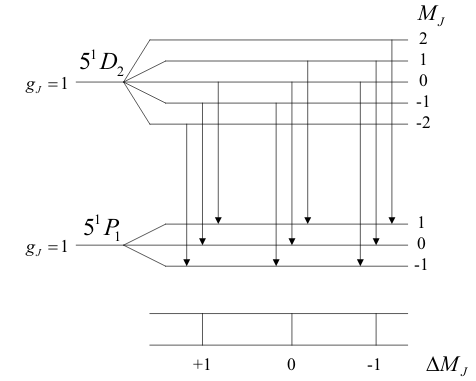
\includegraphics[height=4cm]{content/pictures/cdrot.png}
  \caption{Aufspaltung der roten Spektrallinie.\cite{zeeman}}
  \label{fig:cdrot}
\end{figure}
\begin{figure}[htb]
  \centering
  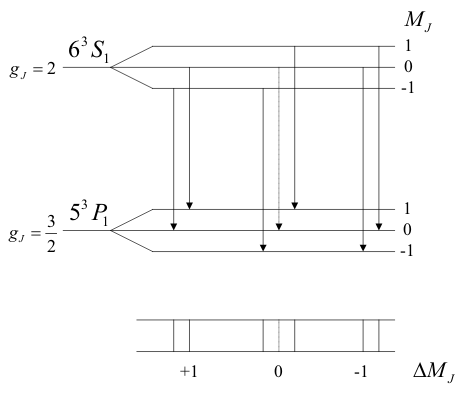
\includegraphics[height=4cm]{content/pictures/cdblau.png}
  \caption{Aufspaltung der blauen Spektrallinie.\cite{zeeman}}
  \label{fig:cdblau}
\end{figure}
In Tabelle \ref{tab:Lande_rot} sind die theoretisch berchneten Landé-Faktoren für den Übergang $^1P_1 \leftrightarrow ^1\!\!D_2$,
unter zu Hilfename von Formel \eqref{eqn:azee} gelistet.
\begin{table}
	\centering
  \caption{Landé-Faktoren für den Übergang $^1P_1 \leftrightarrow ^1\!\!D_2$.}
	\label{tab:Lande_rot}
	\begin{tabular}{cccccc}
		\toprule
		{} & \multicolumn{2}{c}{${}^1P_1$}  & \multicolumn{2}{c}{${}^1D_2$}  & $^1P_1 \leftrightarrow ^1\!\!D_2$ \\
		\midrule
		 Übergang &   $m_1$  & $g_{1}$ & $m_2$ & $ g_2$  & $g_{12}$  \\
		\midrule
		& 2 & 1 & 1 & 1 & 1\\
		$\sigma^-$ & 1 & 1 & 0 & 1 & 1\\
		& 0 & 1 & -1 & 1 & 1\\
		\midrule
		& 1 & 1 & 1 & 1 & 0\\
		$\pi$ & 0 & 1 & 0 & 1 & 0\\
		& -1 & 1 & -1 & 1 & 0\\
		\midrule
		& 0 & 1 & 1 & 1 & -1\\
		$\sigma^+$ & -1 & 1 & 0 & 1 & -1\\
		& -2 & 1 & -1 & 1 & -1\\\bottomrule
	\end{tabular}
  \end{table}
  Die Landé-Faktoren für den Übergang $^3S_1\leftrightarrow ^3\!\!P_1$ stehen in Tabelle \ref{tab:Lande_blau}.

  \begin{table}
  \caption{Landé-Faktoren für den Übergang $^3S_1\leftrightarrow ^3\!\!P_1$.} %Landé
	\label{tab:Lande_blau}
	\centering
  \renewcommand{\arraystretch}{1.2}
  \begin{tabular}{cccccc}
		\toprule
    & \multicolumn{2}{c}{${}^3S_1$}  & \multicolumn{2}{c}{${}^3P_2$} \\
		\midrule
    Übergang & $m_1$  & $g_{1}$ & $m_2$ & $ g_2$ & $g_{12}$\\
		\midrule
		\multirow{2}{*}{$\sigma^-$} & +1 & 2 & 0 & $\frac{3}{2}$& 2\\
		& 0 & 2 & -1 & $\frac{3}{2}$ & $\frac{3}{2}$\\
		\midrule
		& +1 & 2 & +1 & $\frac{3}{2}$ & $\frac{1}{2}$\\
		$\pi$ & 2 & 2 & 0 & $\frac{3}{2}$ & 0 \\
		& -1 & 2 & -1 & $\frac{3}{2}$ & -$\frac{1}{2}$\\
		\midrule
		\multirow{2}{*}{$\sigma^+$} & 0 & 2 & 1 & $\frac{3}{2}$ & -$\frac{3}{2}$\\
		& -1 & 2 & 0 & $\frac{3}{2}$& -2\\
		\bottomrule
	\end{tabular}
\end{table}
\FloatBarrier

\subsection{Eichung des Elektromagneten}
Um im Folgendem die gemessenen Daten zu verwerten muss das B-Feld kalibriert werden.
Dazu werden an die in Tabelle \ref{tab:b} zu sehenden Messdaten, mittels scipy \cite{scipy} eine Regressionsfunktion der Form 
\begin{equation*}
  B = a_0 + a_1I + a_2I^2 + a_3I^3 + a_4I^4
\end{equation*}
gefittet.Dabei ist $I$ der Strom und $B$ die Magnetfeldstärke.
Mit der Ausgleichsrechnung werden die Werte der Regression auf
\begin{align*}
  a_0&=\SI{1.56(45)e-2}{\tesla}\\
  a_1&=\SI{5.60(28)e-2}{\tesla\per\ampere}\\
  a_2&=\SI{0.10(5)e-2}{\tesla\per\ampere\squared}\\
  a_3&=\SI{-4(3)e-5}{\tesla\per\ampere\cubed}\\
  a_4&=\SI{-6(8)e-7}{\tesla\per\ampere\tothe{4}}
\end{align*}
bestimmt.
Messdaten und Fit sind in Abbildung \ref{fig:eichung} dargestellt.
Durch diese Funktion kann das angelegte B-Feld bestimmt werden.

\begin{table}
	\centering
	\caption{Gemessenes Magnetfeld abhängig vom angelegten Strom.}
	\label{tab:b}
	\begin{tabular}{
		S[table-format=2]
		S[table-format=4]
		}
	\toprule
		{$I$\;/\;\si{\ampere}} & {$B$\;/\;\si{\milli\tesla}} \\
	\midrule
		 1 &  69 \\
         2 &  138 \\
         3 &  191 \\
         4 &  253 \\
         5 &  312 \\
         6 &  379 \\
         7 &  442 \\
         8 &  506 \\
         9 &  567 \\
         10 &  629 \\
         11 &  687 \\
         12 &  748 \\
         13 &  802 \\
         14 &  853 \\
         15 &  909 \\
         16 &  955 \\
         17 &  995 \\
         18 &  1030 \\
         19 &  1060 \\
         20 &  1093 \\
	\bottomrule
	\end{tabular}
\end{table}
\begin{figure}[htb]
  \centering
  \includegraphics[width=\textwidth]{build/eichung.pdf}
  \caption{Die Messwerte zur Kalibration des $B$-Feldes und der Fit.}
  \label{fig:eichung}
\end{figure}
\FloatBarrier

\subsection{Berechnung der Landé-Faktoren}
Aus der Verschiebung der Wellenlänge $\delta\lambda$ werden die Landé-Faktoren bestimmt.
Diese werden aus der Formel
\begin{equation}
  \label{eqn:lamb_versch}
  \delta\lambda=\frac{1}{2}\frac{\delta s}{\Delta s}\Delta\lambda_\text{D}
\end{equation}
errechnet.
Hierbei ist $\Delta s$ der Abstand der Spektrallinien ohne B-Feld und $\delta s$ der Abstand zwischen den im B-Feld aufgespaltenen Linien.
Mit \eqref{eqn:disp} wird $\Delta\lambda_\text{D}$ berechnet, diese Werte sind in Tabelle \ref{tab:disp} einzusehen.
Aus \eqref{eqn:lamb_versch} lässt sich jetzt die Energieverschiebung $\Delta E$ bestimmen:
\begin{align}
  \label{eqn:DE}
  \Delta E &= \left |\frac{\partial E}{\partial \lambda}\right |\delta \lambda\nonumber\\
  &=\frac{\symup{hc}}{\lambda^2}\delta\lambda,
\end{align}
wobei $\symup{c}$ die Lichtgeschwindigkeit und $\symup{h}$ das Plank'sche Wirkungsquantum ist.
\begin{table}
	\centering
	\caption{Dispersionsgebiet der Lummer-Gehrcke-Platte.}
	\label{tab:disp}
	\begin{tabular}{
		S[table-format=2.2]
		S[table-format=3.1]
		}
	\toprule
		{$\Delta\lambda_\text{D}$\;/\;\si{\pico\meter}} & {$\lambda$\;/\;\si{\nano\meter}} \\
	\midrule
		 48,91 &  643,8 \\
         26,95 &  480,0 \\
	\bottomrule
	\end{tabular}
\end{table} 



\subsubsection{Rote Linie}
In Abbildung \ref{fig:rot_pi_0A} sind die Spektrallinien mit Wellenlänge $\lambda=\SI{643.8}{\nano\meter}$ bei ausgeschaltetem Magnetfeld zu sehen.
Bei einem Magnetfeld der Stärke $B=\SI{0.63(7)}{\tesla}$ ist in Abbildung \ref{fig:rot_pi_10A} keine Aufspaltung der Spektrallinien zu erkennen,
was nach der Theorie zu erwarten war.
\begin{figure}[htb]
  \centering
  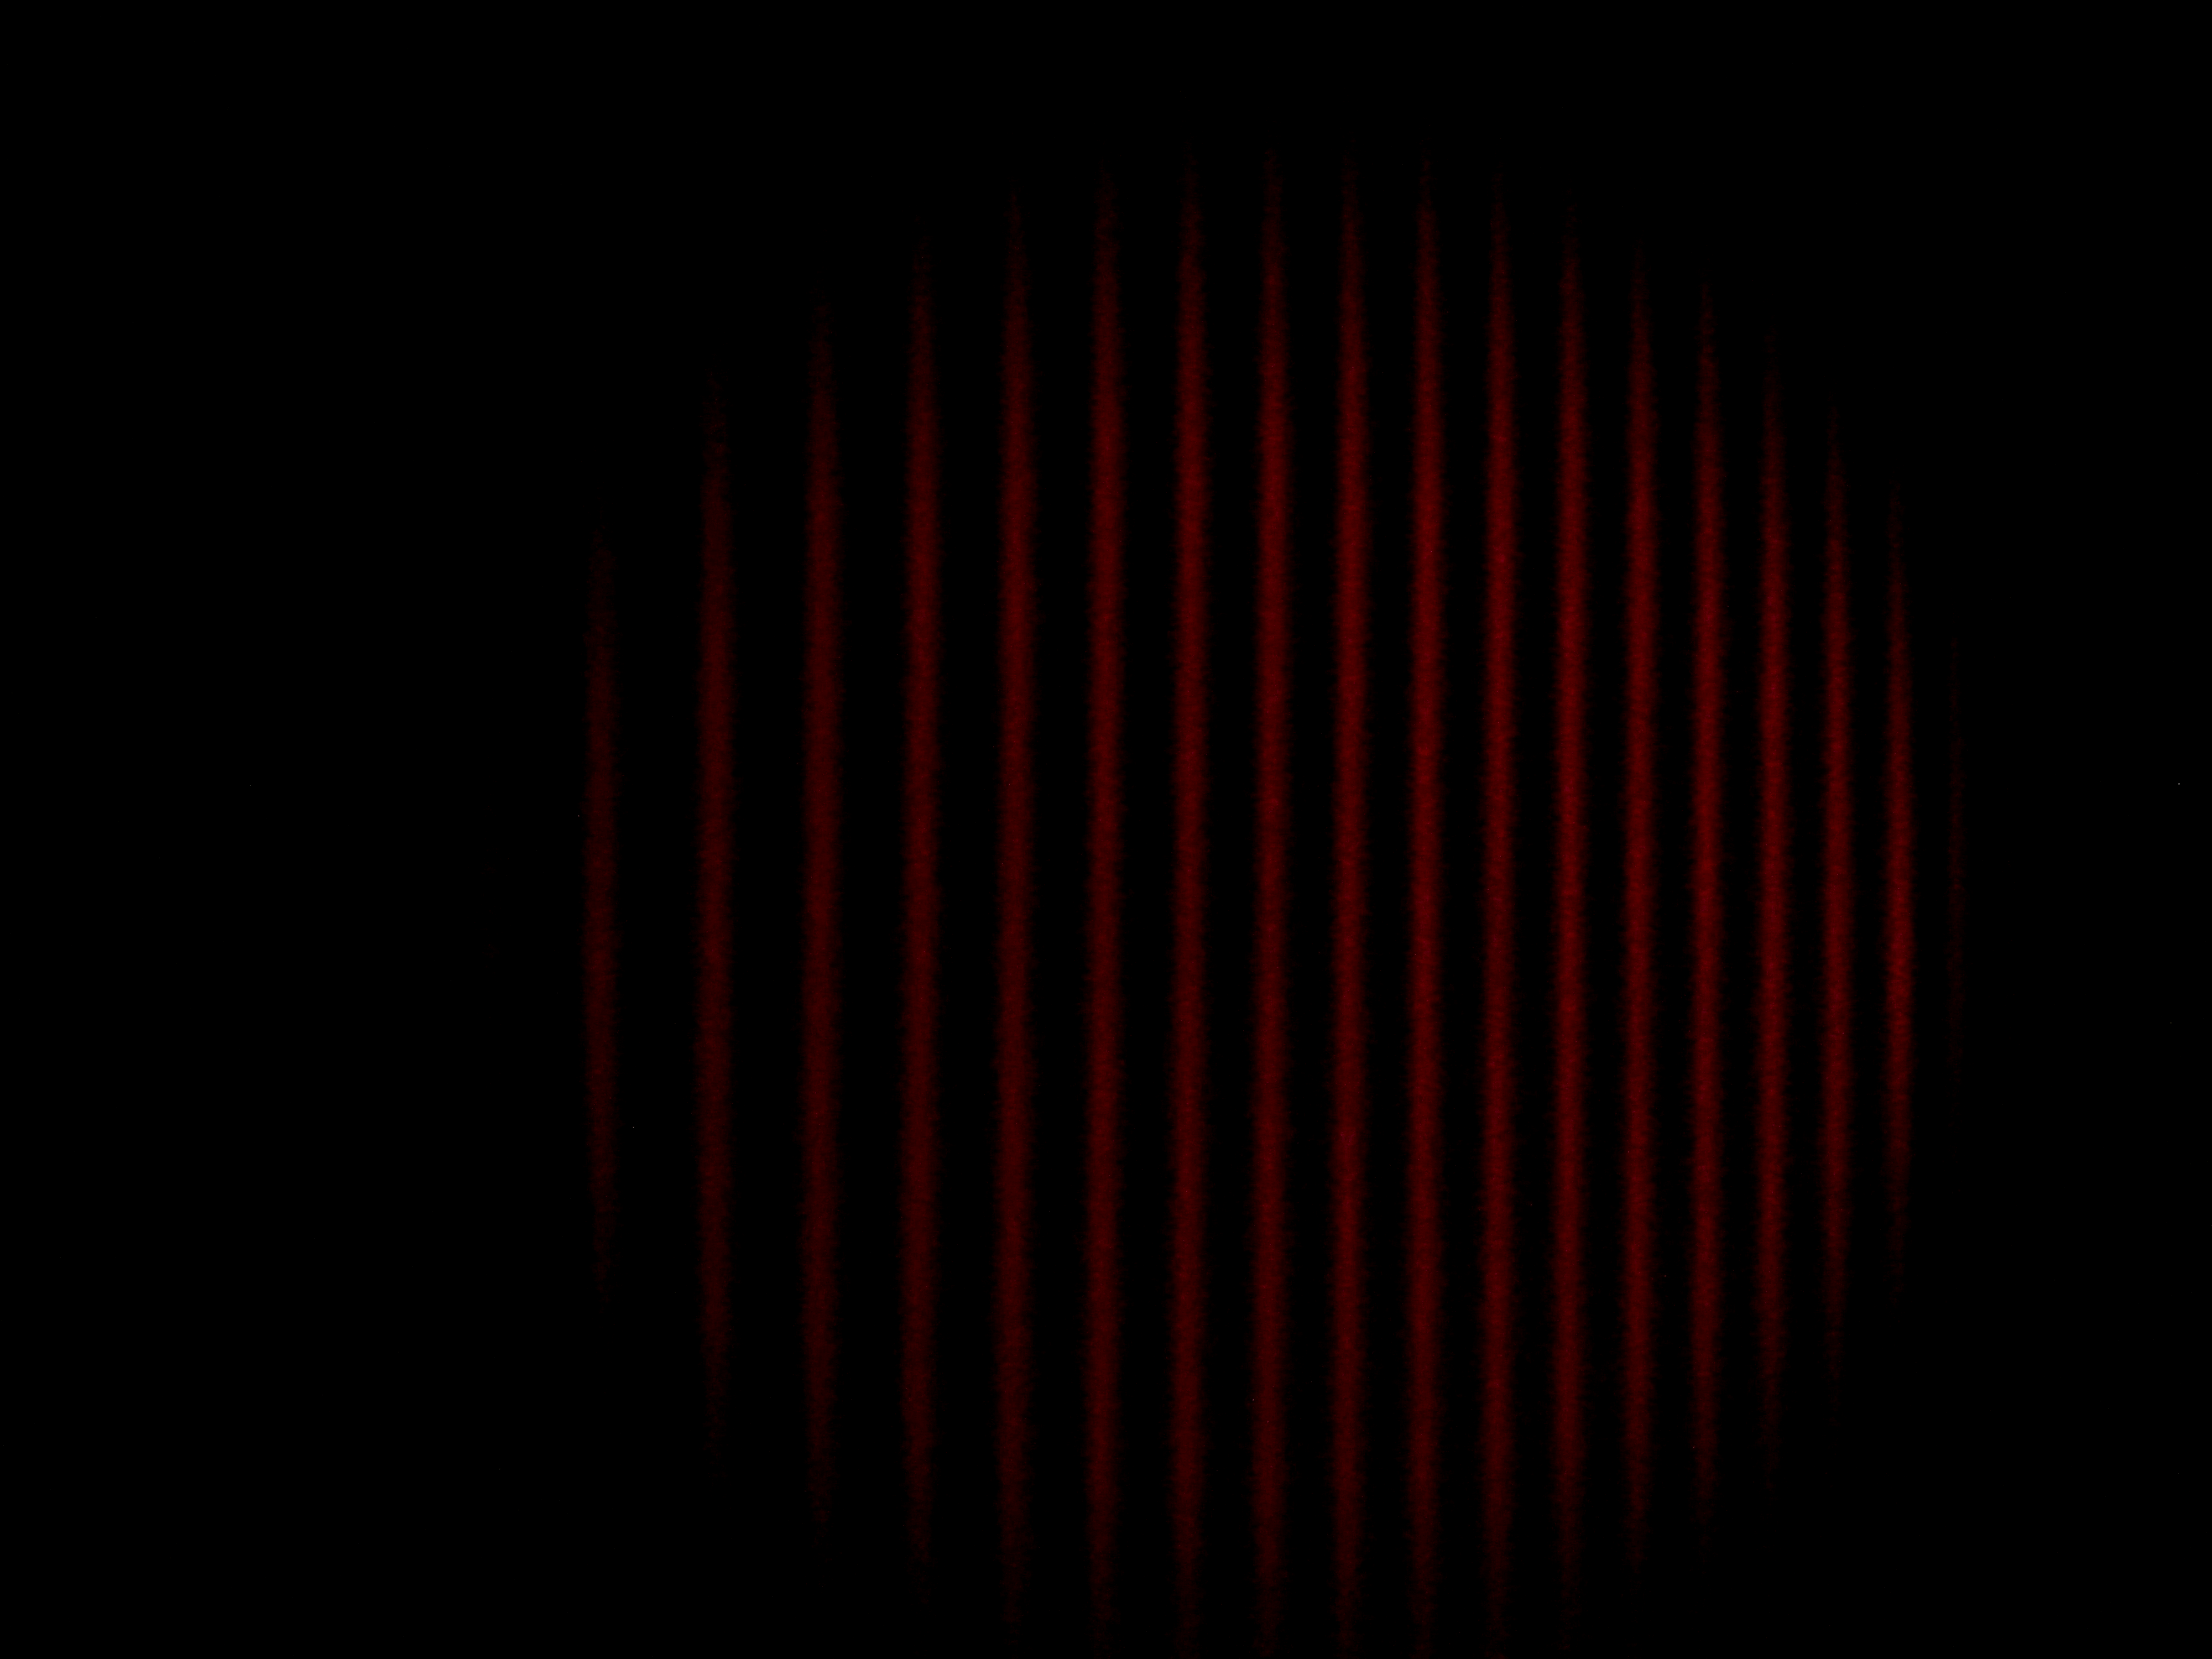
\includegraphics[height=8cm]{content/pictures/rot_pi_0A.png}
  \caption{Spektrallinie für $\lambda=\SI{643.8}{\nano\meter}$.}
  \label{fig:rot_pi_0A}
\end{figure}
\begin{figure}[htb]
  \centering
  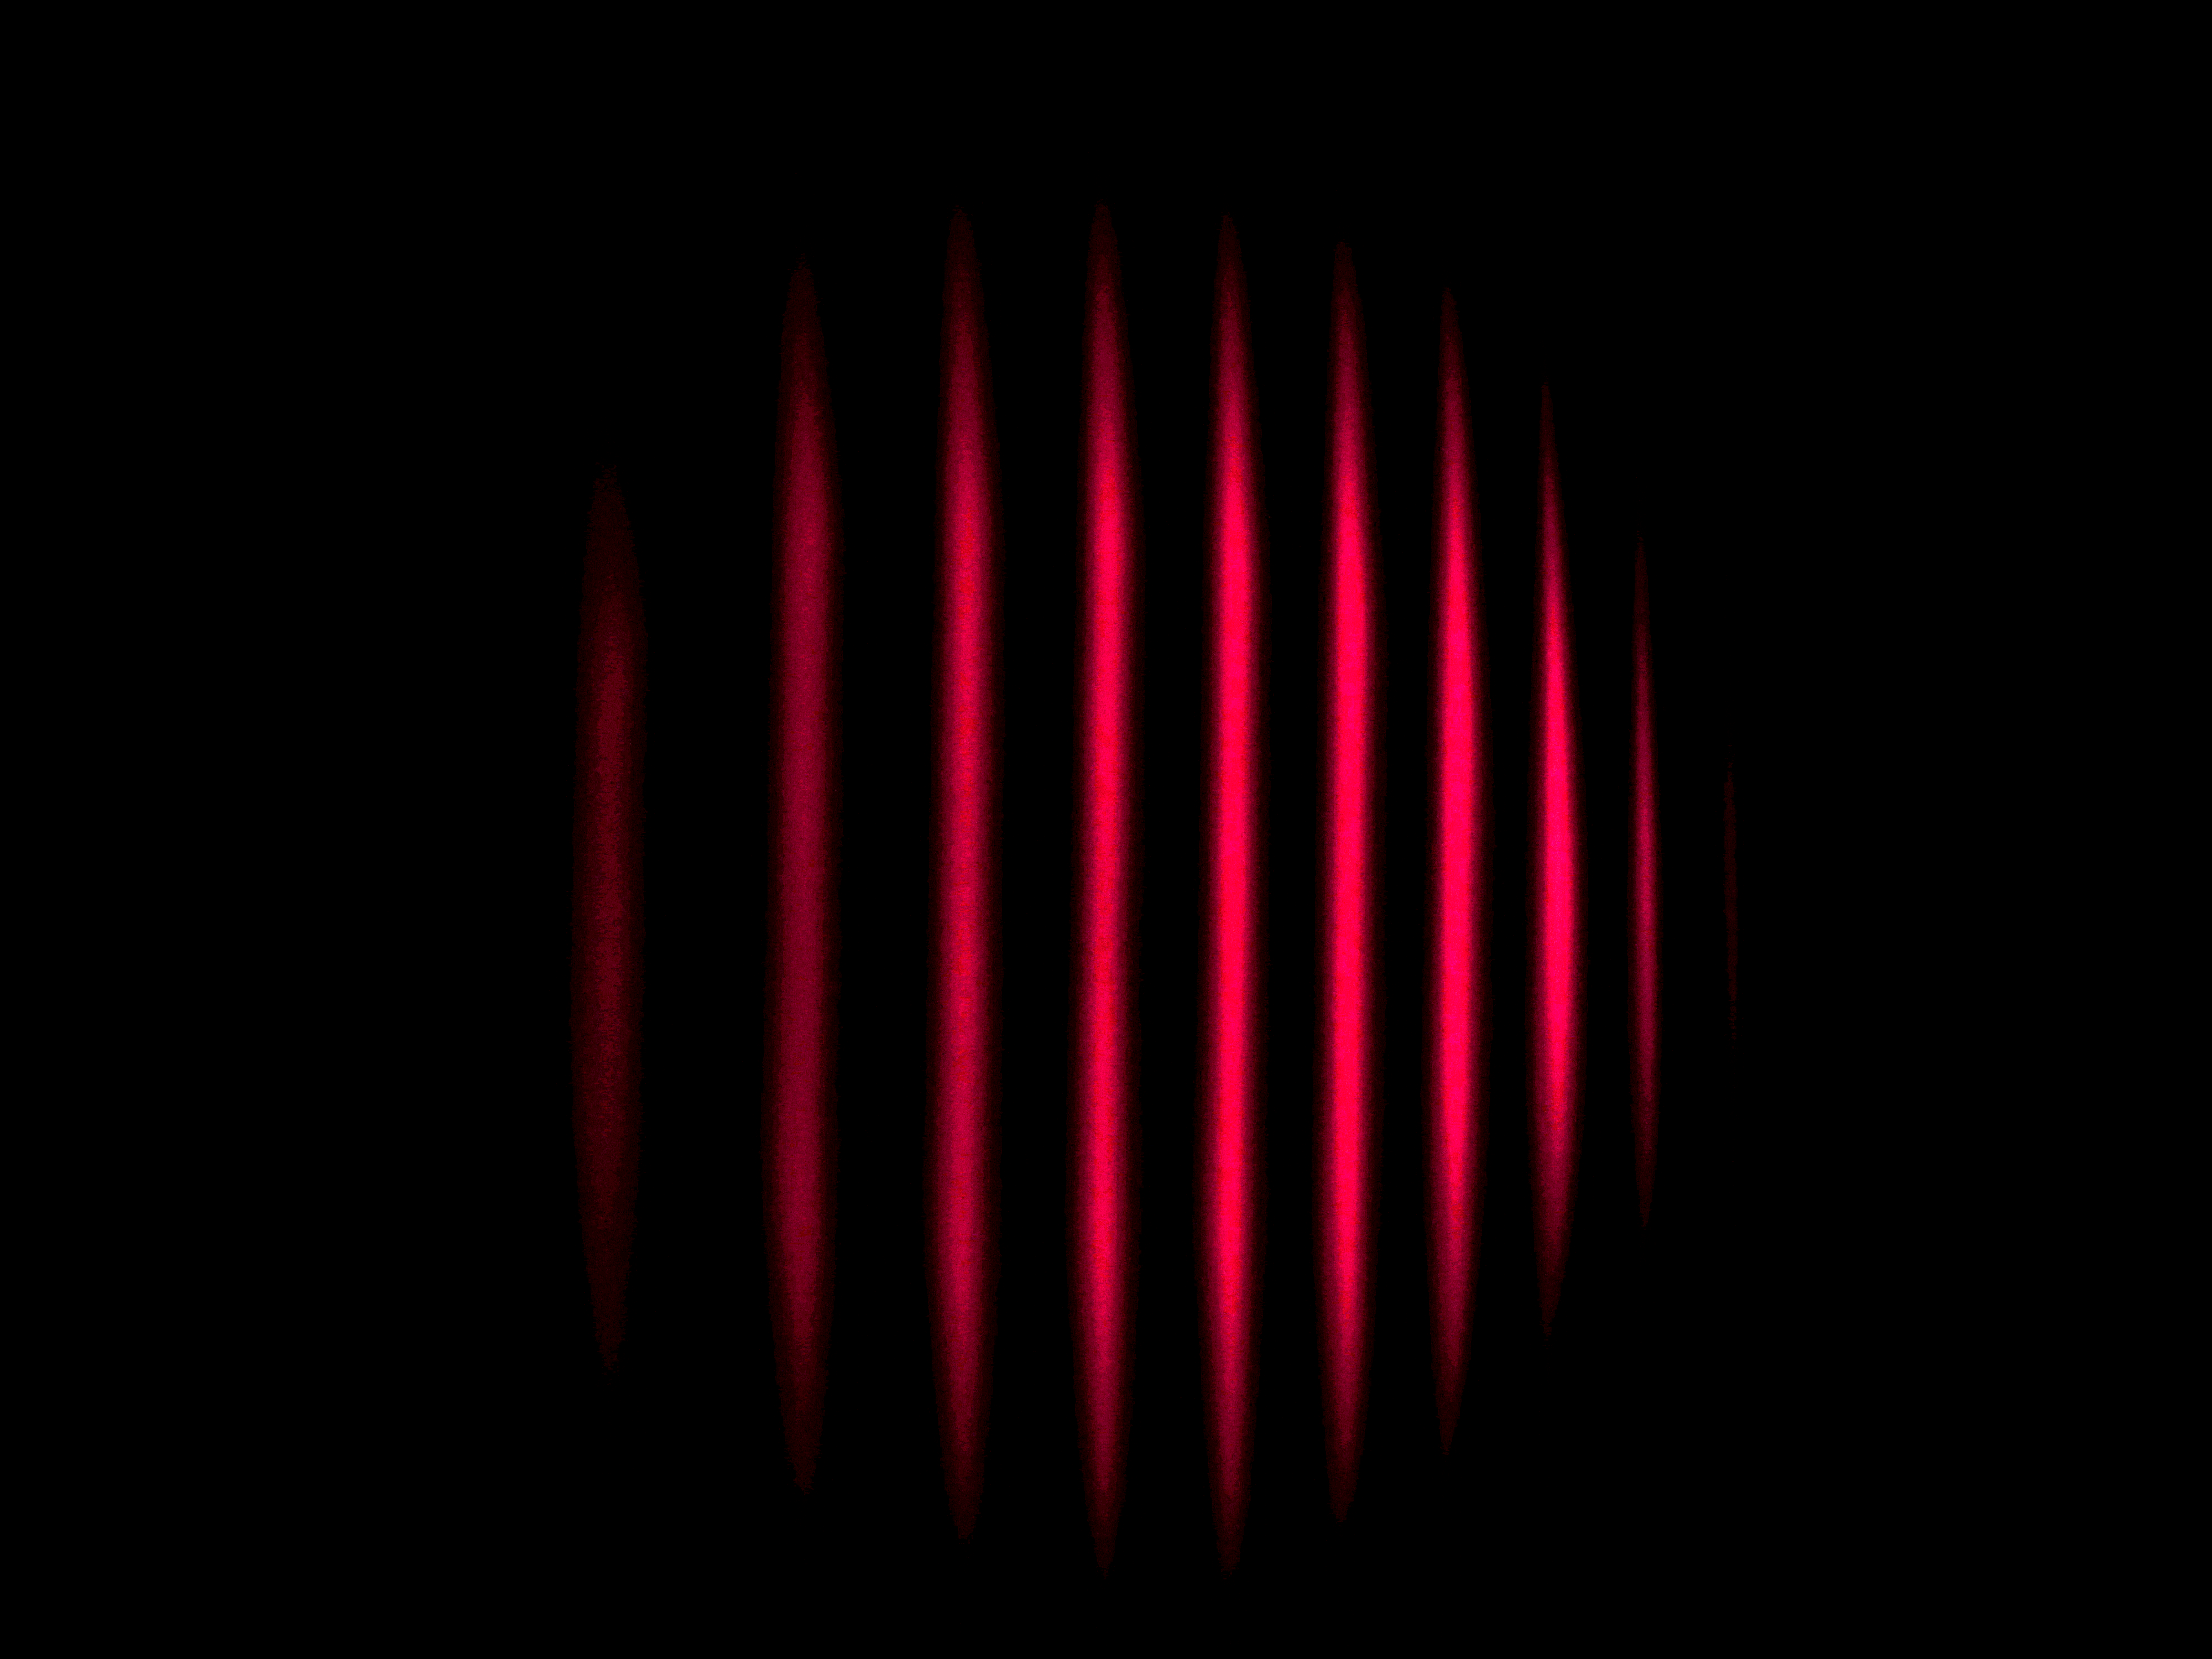
\includegraphics[height=8cm]{content/pictures/rot_pi_10A.png}
  \caption{$\pi$-Linie für $\lambda=\SI{643.8}{\nano\meter}$.}
  \label{fig:rot_pi_10A}
\end{figure}
In Abbildung \ref{fig:rot_sigma_0A} ist das Interferenzbild der Spektrallinie zu sehen, die durch einen \SI{90}{\degree} Polarisationsfilter geht.
Nach Einschalten des Magnetfelds auf $B=\SI{0.63(7)}{\tesla}$ wird das Bild aus Abbildung \ref{fig:rot_sigma_10A} aufgenommen.
\begin{figure}[htb]
  \centering
  \includegraphics[height=8cm]{content/pictures/rot_sigma_0A.png}
  \caption{Spektrallinie für $\lambda=\SI{643.8}{\nano\meter}$ nach dem Polarisationsfilter.}
  \label{fig:rot_sigma_0A}
\end{figure}
\begin{figure}[htb]
  \centering
  \includegraphics[height=8cm]{content/pictures/rot_sigma_10A.png}
  \caption{$\sigma$-Linie für $\lambda=\SI{643.8}{\nano\meter}$ bei $B=\SI{0.63(7)}{\tesla}$.}
  \label{fig:rot_sigma_10A}
\end{figure}
Durch imageio \cite{imageio} werden die Bilder verarbeitet und die Distanz zwischen den Intensitätsmaxima gemessen.
Die von dem Programm erfassten Daten sind in den Abbildung \ref{fig:rot_sigma_0A_plot} und \ref{fig:rot_sigma_10A_plot} zu sehen.
\begin{figure}[htb]
  \centering
  \includegraphics[height=10cm]{build/rot_sigma_0A.pdf}
  \caption{Rotwerte des Interferenzbildes für $\lambda=\SI{643.8}{\nano\meter}$ bei ausgeschaltetem Magnetfeld und einem \SI{90}{\degree} Polarisationsfilter.}
  \label{fig:rot_sigma_0A_plot}
\end{figure}
\begin{figure}[htb]
  \centering
  \includegraphics[height=10cm]{build/rot_sigma_10A.pdf}
  \caption{Rotwerte des Interferenzbildes für $\lambda=\SI{643.8}{\nano\meter}$ bei $B=\SI{0.63(7)}{\tesla}$ und einem \SI{90}{\degree} Polarisationsfilter.}
  \label{fig:rot_sigma_10A_plot}
\end{figure}
Die Daten sind in Tabelle~\ref{tab:rot_sigma} zusammengefasst.
Der Mittelwert der Landé-Faktoren wird auf
\begin{equation}
  \label{eqn:g_rot_sigma}
  \bar{g}_{\text{rot},\sigma}=\num{0.99(11)}
\end{equation}
bestimmt, dazu werden die Daten mit  
\begin{equation}
  \label{eqn:g}
  g=m_1 \cdot g(L_1, S_1, J_1) - m_2 \cdot g(L_2, S_2, J_2)=\frac{\Delta E}{\mu_\text{B}B},
\end{equation}
welche aus Formel \eqref{eqn:azee} abgeleitet wird, ausgewertet. Die Energiedifferentz $\Delta E$ ergibt sich aus den 
Abbildungen nach Formel \eqref{eqn:DE} mit \eqref{eqn:lamb_versch}.
\input{build/rot_sigma.tex}
\FloatBarrier

\subsubsection{Blaue Linie}
Bild \ref{fig:blau_pi_0A} zeigt die Spektrallinie für $\lambda=\SI{480}{\nano\meter}$ bei ausgeschaltetem B-Feld.
In Abbildung \ref{fig:blau_pi_6A} ist die Aufspaltung der $\sigma-$Linien bei $B=\SI{0.37(3)}{\tesla}$ zu sehen.
\begin{figure}[htb]
  \centering
  \includegraphics[height=8cm]{content/pictures/blau_pi_0A.JPG}
  \caption{Interferenzbild für $\lambda=\SI{480}{\nano\meter}$ bei ausgeschaltetem Magnetfeld.}
  \label{fig:blau_pi_0A}
\end{figure}
\begin{figure}[htb]
  \centering
  
\includegraphics[height=8cm]{content/pictures/blau_pi_6A.JPG}
  \caption{$\sigma-$Linie für $\lambda=\SI{480}{\nano\meter}$ bei $B=\SI{0.37(3)}{\tesla}$.}
  \label{fig:blau_pi_6A}
\end{figure}
Die relevanten Daten sind in Abbildungen \ref{fig:blau_pi_0A_plot} und \ref{fig:blau_pi_6A_plot} einzusehen.
Für die Rechnung wichtige Werte stehen in Tabelle \ref{tab:blau_pi}.
\begin{figure}[htb]
  \centering
  \includegraphics[height=10cm]{build/blau_pi_0A.pdf}
  \caption{Blauwerte des Interferenzbildes für $\lambda=\SI{480}{\nano\meter}$ bei ausgeschaltetem Magnetfeld.}
  \label{fig:blau_pi_0A_plot}
\end{figure}
\begin{figure}[htb]
  \centering
  
\includegraphics[height=10cm]{build/blau_pi_6A.pdf}
  \caption{Blauwerte des Interferenzbildes für $\lambda=\SI{480}{\nano\meter}$ bei $B=\SI{0.37(3)}{\tesla}$.}
  \label{fig:blau_pi_6A_plot}
\end{figure}
Der Mittelwert lässt sich auf
\begin{equation}
  \label{eqn:g_blau_sigma}
  \bar{g}_{\text{blau},\sigma}=\num{1.82(13)}
\end{equation}
bestimmen.
\input{build/blau_pi.tex}

Zum Schluss werden die $\pi-$Linien ohne (Abb. \ref{fig:blau_sigma_0A}) und mit (Abb. \ref{fig:blau_sigma_20A}) eingeschaltetem Magnetfeld untersucht.
\begin{figure}[htb]
  \centering
  
\includegraphics[height=8cm]{content/pictures/blau_sigma_0A.JPG}
  \caption{Interferenzbild für $\lambda=\SI{480}{\nano\meter}$ bei ausgeschaltetem Magnetfeld.}
  \label{fig:blau_sigma_0A}
\end{figure}
\begin{figure}[htb]
  \centering
  \includegraphics[height=8cm]{content/pictures/blau_sigma_20A.JPG}
  \caption{Interferenzbild für $\lambda=\SI{480}{\nano\meter}$ bei $B=\SI{1.1(4)}{\tesla}$.}
  \label{fig:blau_sigma_20A}
\end{figure}
Dazu werden mit den Daten aus Abbildungen \ref{fig:blau_sigma_0A_plot} und \ref{fig:blau_sigma_20A_plot} die Berechnungen wiederholt.
\begin{figure}[htb]
  \centering
  
\includegraphics[height=10cm]{build/blau_sigma_0A.pdf}
  \caption{Blauwerte des Interferenzbildes für $\lambda=\SI{480}{\nano\meter}$ bei $B=0$.}
  \label{fig:blau_sigma_0A_plot}
\end{figure}
\begin{figure}[htb]
  \centering
  \includegraphics[height=10cm]{build/blau_sigma_20A.pdf}
  \caption{Blauwerte des Interferenzbildes für $\lambda=\SI{480}{\nano\meter}$ bei $B=\SI{1.1(4)}{\tesla}$.}
  \label{fig:blau_sigma_20A_plot}
\end{figure}
Die errechneten Werte befinden sich in Tabelle \ref{tab:blau_sigma}.
Der Mittelwert des Landé-Faktor ist damit
\begin{equation}
\label{eqn:g_blau_pi}
\bar{g}_{\text{blau},\pi}=\num{0.43(16)}.
\end{equation}
\input{build/blau_sigma.tex}
\FloatBarrier